\section{Rechenzeit}
\label{sec:rechenzeit}
Die Rechenzeit bezieht sich auf die Zeit, die benötigt wird, um aus einer Schachposition den besten Zug zu berechnen.
Je kürzer die Zeit, desto besser die Auswertung.
Diese Metrik wird nicht mit \gls{glos:stockfish} verglichen, da dies sehr unrealistisch wäre.
Der Vergleich beschränkt sich auf die verschiedenen Eigenimplementierungen, um festzustellen, welche Ansätze die grössten Zeitersparnisse bringen.

\subsection{Testaufbau}
Alle Tests wurden als \gls{glos:JUnit}-Tests konzipiert.
Für die Tests wurden zwölf Schachpositionen ausgewählt: Sieben stammten aus \gls{glos:lichess} Puzzles, vier wurden von einer KI generiert und manuell überprüft, und eine wurde manuell erstellt.
Es wurde ein \texttt{@ParameterizedTest} erstellt, der die erwähnten Positionen als \texttt{@MethodSource} verwendet.
So wird die Testlogik nur einmal geschrieben und für jede Schachposition ausgeführt.
Alle Tests laufen sequentiell ab, damit sie sich nicht gegenseitig Ressourcen wegnehmen.

Der \gls{glos:JUnit}-Test holt dynamisch alle Minimax-Algorithmus Implementierungen.
Die gewünschten Evaluationsstrategiekombinationen können mittels \texttt{CompositeEvaluationStrategy} erstellt werden.
\begin{lstlisting}[
    language = JavaIntelliJ,
    caption={CompositeEvaluationStrategy - Aufruf Beispiel},
    label={lst:composite-eval-strategy-call-example}
]
var strategy = CompositeEvaluationStrategy.builder().add(new MateAwareEvaluation()).add(new MaterialEvaluation()).build();
\end{lstlisting}


Dieser Test verwendet die gleichen Kombinationen der Evaluationsstrategien wie der Zugqualitätstest, jedoch kombiniert mit allen Algorithmen, und führt sie für die parametrierte Position aus.
Zusätzlich kann noch die Suchtiefe für jede Kombination eingestellt werden.
Für die meisten Kombinationen wird eine Tiefe von 5 eingestellt.
Die Alpha-Beta-Pruning Implementierungen zeigten sich bei vorherigen Ausführungen performanter und werden aus diesem Grund auf die Tiefe 7 eingestellt. \\
Alle Messungen werden zehnmal durchgeführt und es wird der Median aller Durchführungen berechnet.
Somit sollten grosse Ausreisser die Resultate nicht stark beeinflussen.

Der Test stellt ausserdem sicher, dass alle wiederholten Messungen sowie alle Algorithmen, die dieselben Auswertungsstrategien verwenden, zu denselben Ergebnissen führen.
Durch diese Prüfung wird sichergestellt, dass alle Zeitunterschiede gültig sind.

Die Testergebnisse werden in Dateien gespeichert, die zur Erstellung von Diagrammen verwendet werden.

\newpage

\subsection{Testresultate}
Für jede Position wurde ein \gls{glos:plantuml}-Diagramm erstellt mit den Algorithmen, Zugtiefen und Rechenzeiten.
Alle Diagramme befinden sich im Anhang unter Rechenzeit Daten~\ref{ch:performance_data} und sehen wie folgt aus.

\begin{figure}[H]
    \centering
    
\includegraphics[width=\linewidth]{evaluation/report/performance/complexPositionWithManyOptions/ComplexPositionWithManyOptions}
    \caption{Rechenzeiten für die erste getestete Schachposition}
    \label{fig:rechenzeiten-fuer-erste-position}
\end{figure}

Für die vertikale Achse wurde eine \gls{glos:logskala} zur Basis 10 verwendet, da sich die Rechenzeiten pro Tiefe stark unterscheiden.
Bei einer linearen Skala könnten entweder die kleineren Werte nicht verglichen werden, oder die Diagramme müssten sehr hoch sein.

Wie vorher erwähnt wurden für die Zugtiefen 6 und 7 nur die Algorithmen mit der Alpha-Beta-Pruning Optimierung (mit und ohne Caching) evaluiert.
Der Grund dafür ist der grosse Unterschied der Rechenzeiten - der Test würde viel zu lange dauern.

Für die grösste gemeinsam berechenbare Zugtiefe wurde noch eine Tabelle erstellt, welche die relativen Rechengeschwindigkeiten zum nicht optimierten Algorithmus aufzeigt.
Die Zahlen geben den Geschwindigkeitsmultiplikator im Vergleich zum ursprünglichen Algorithmus an - die Zahl 2 steht also für die doppelte Geschwindigkeit bzw.\ die Hälfte der erforderlichen Rechenzeit.
\begin{table}[H]
    \centering
    \resizebox{\textwidth}{!}{%
        \begin{tabular}{|p{8cm}|*{5}{r|}}
    \hline
    & \multicolumn{5}{c|}{\textbf{Median performance gain multiplier}} \\
    \cline{2-6}
    \multirow{-2}{*}{\parbox{8cm}{\centering\textbf{Strategy}}} & \multicolumn{1}{r|}{\textbf{MiniMaxAlphaBetaSequentialWithCache}} & \multicolumn{1}{r|}{\textbf{MiniMaxAlphaBetaSequential}} & \multicolumn{1}{r|}{\textbf{MiniMaxParallelWithCache}} & \multicolumn{1}{r|}{\textbf{MiniMaxParallel}} & \multicolumn{1}{r|}{\textbf{MiniMaxSequentialWithCache}} \\
    \hline
    \rowcolor[HTML]{FFFFFF}
    \textbf{Mate aware piece square evaluation}                 & 686.42                                                            & 522.20                                                   & 14.67                                                  & 7.44                                          & 2.18                                                     \\

    \rowcolor[HTML]{EFEFEF}
    \textbf{Mate aware piece square material evaluation}        & 955.39                                                            & 699.55                                                   & 16.33                                                  & 7.00                                          & 2.56                                                     \\

    \rowcolor[HTML]{FFFFFF}
    \textbf{Mate aware material evaluation}                     & 1139.56                                                           & 836.50                                                   & 14.74                                                  & 7.01                                          & 2.23                                                     \\
    \hline
    \hline
    \rowcolor[HTML]{FFFFFF}
    \textbf{Median}                                             & \textbf{955.39}                                                   & \textbf{699.55}                                          & \textbf{14.74}                                         & \textbf{7.01}                                 & \textbf{2.23}                                            \\

    \hline
\end{tabular}%

    }
    \caption{Medianer Geschwindigkeitsmultiplikator bei Zugtiefe 5}
    \label{tab:medianer-geschwindigkeitsmultiplikator-bei-zugtiefe-5}
\end{table}

Die Werte in der Tabelle sind Medianwerte über alle Schachpositionen.
Die weiteren Tabellen befinden sich im Anhang unter Rechengeschwindigkeitsmultiplikator im Vergleich zu MiniMaxSequential~\ref{sec:performance-gains}.

Für eine kompaktere Darstellung der Evaluationen unterschiedlicher Algorithmen und Strategien wurde pro Zugtiefe noch ein Diagramm erstellt.
Diese Diagramme befinden sich ebenfalls im Anhang, unter Rechenzeiten pro Zugtiefe~\ref{sec:rechenzeiten-pro-zugtiefe}.
Untenstehend noch das Diagramm für die Zugtiefe 5.

\begin{figure}[H]
    \centering
    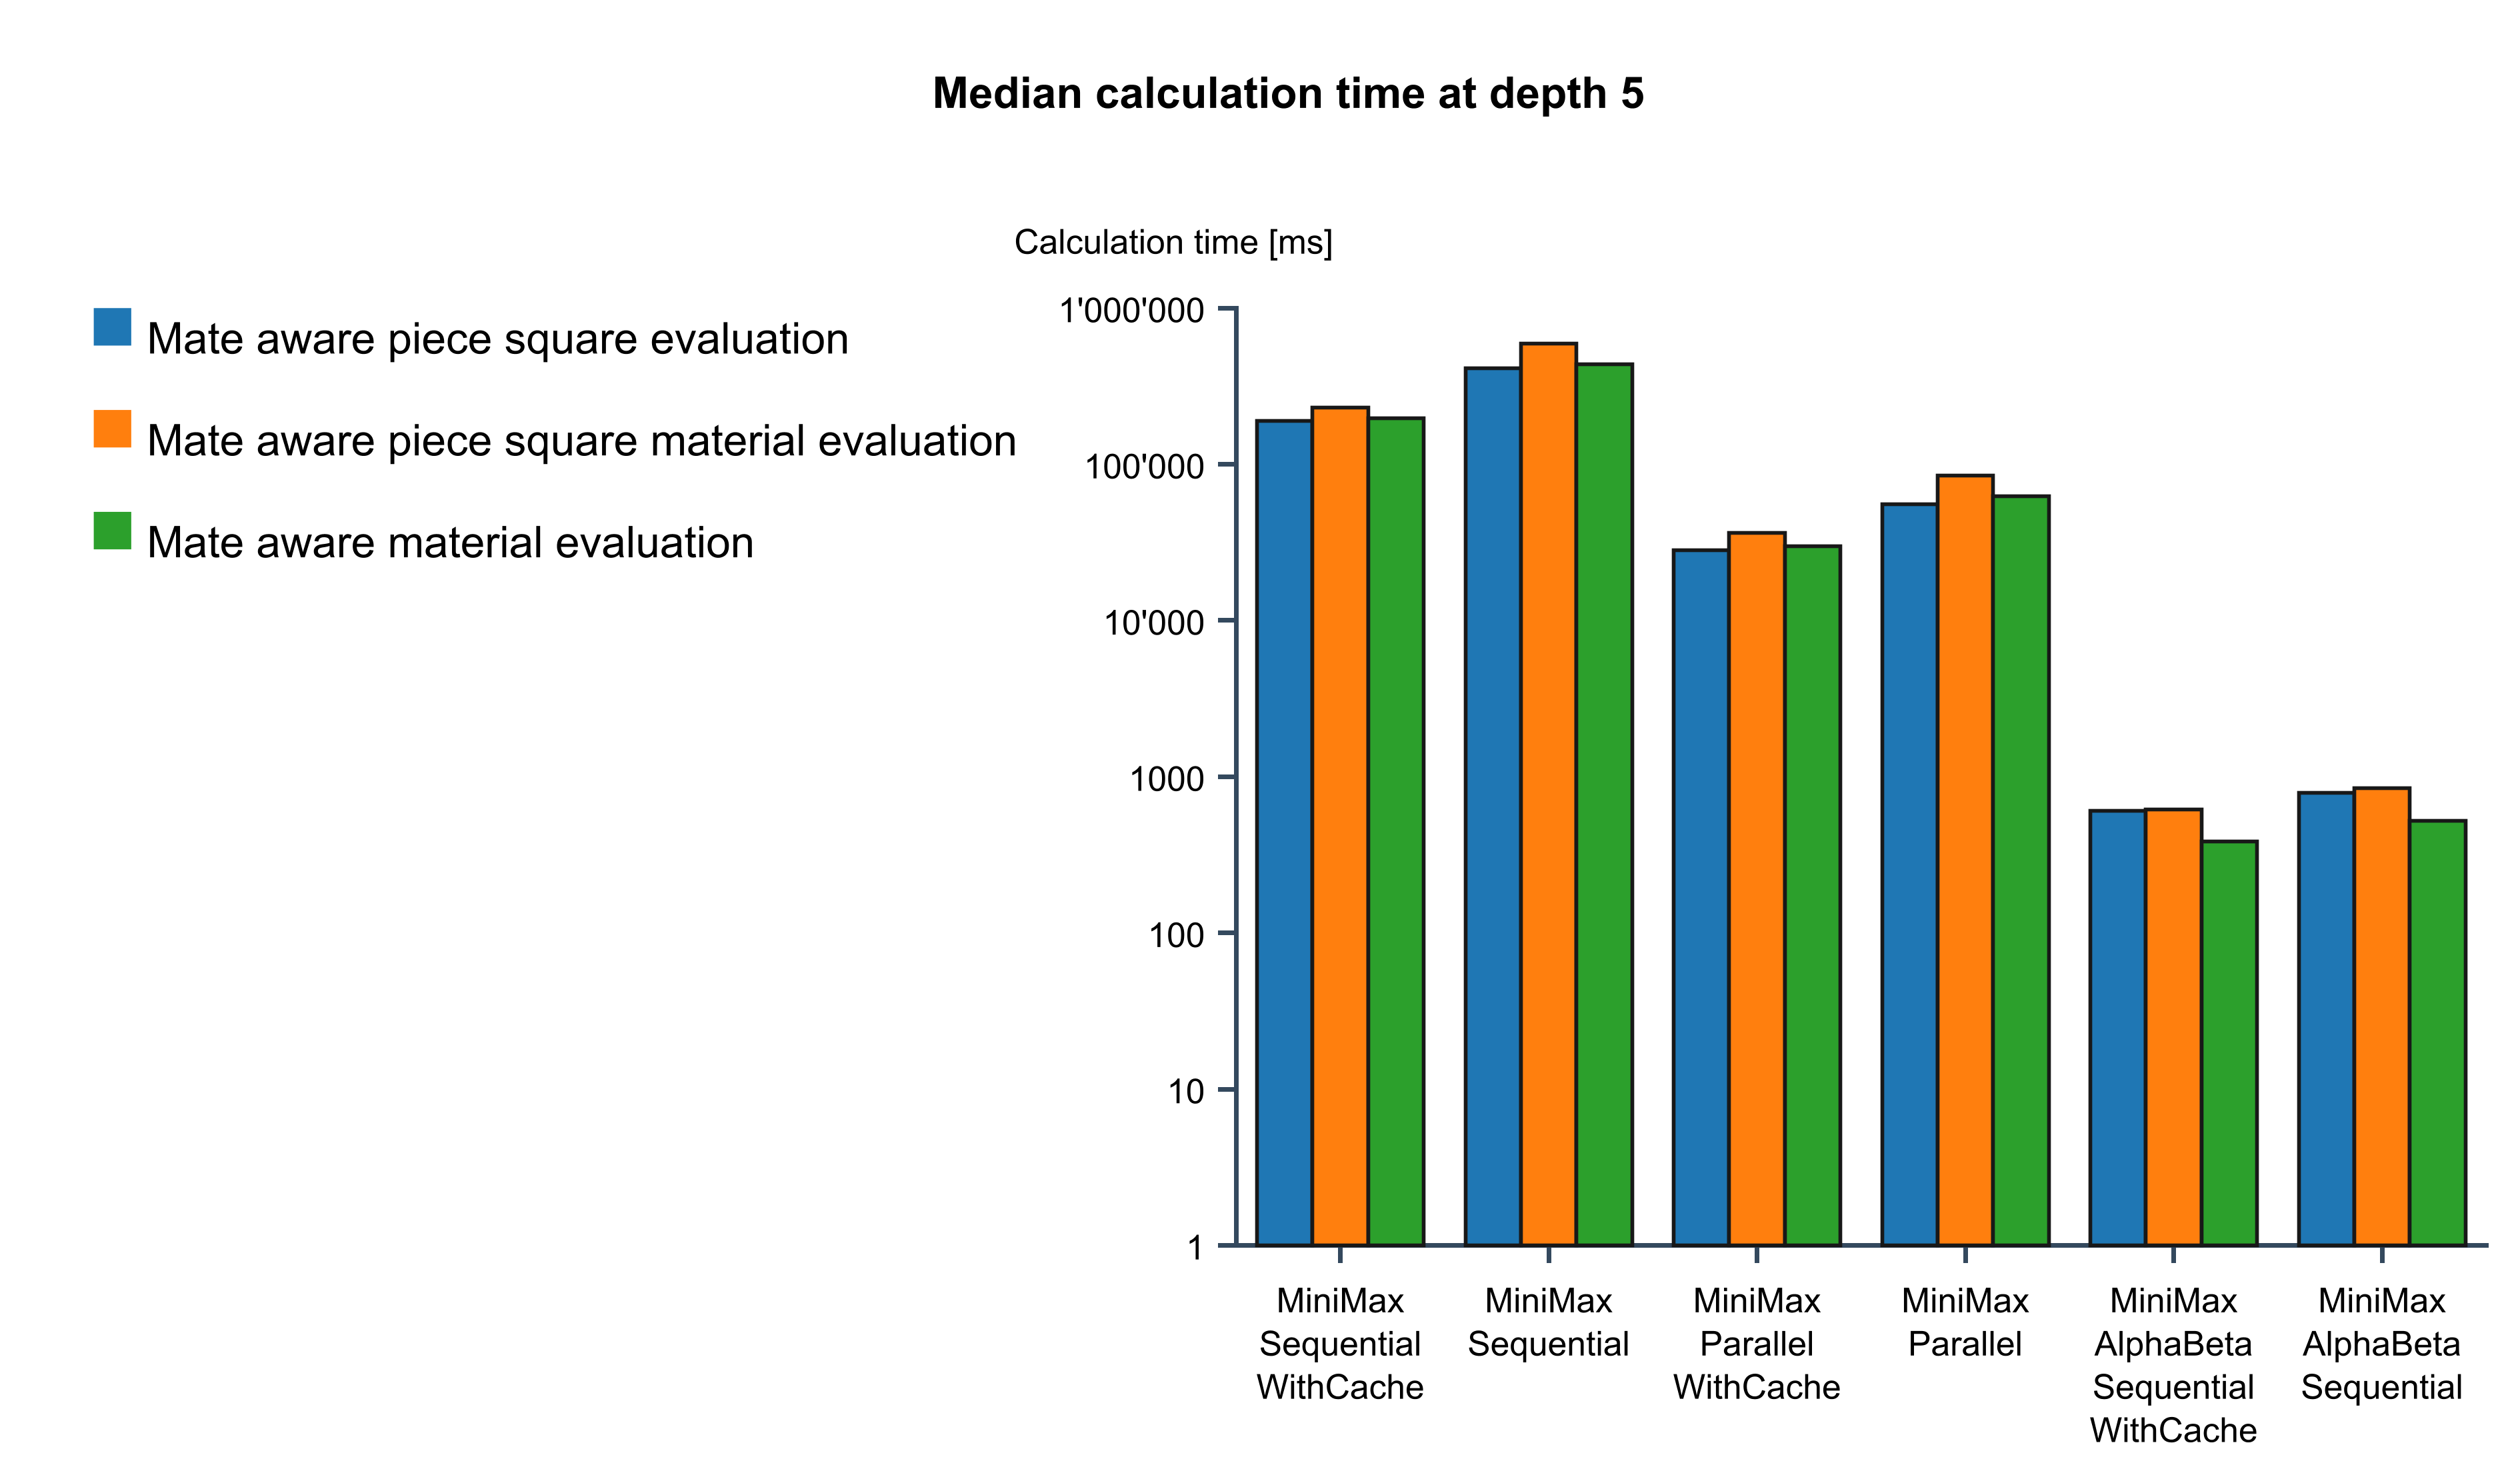
\includegraphics[width=0.9\linewidth]{evaluation/report/performance/performance-at-depth-5-by-strategy}
    \caption{Rechenzeit für Zugtiefe 5}
    \label{fig:rechenzeit-fuer-tiefe-5-pro-strategie}
\end{figure}

\subsection{Interpretation}
Die Messungen zeigen, dass die Alpha-Beta-Pruning-Optimierung den grössten Leistungsgewinn bringt.
Es ist erstaunlich zu sehen, wie viel schneller diese Optimierung im Vergleich zum Caching und zur Parallelisierung ist.

Der Zeitunterschied gegenüber einer einfachen Parallelisierung lässt sich durch die begrenzte Anzahl verfügbarer CPUs erklären.
Allerdings wäre die dafür benötigte Anzahl an CPUs bei grösseren Suchtiefen kaum erreichbar, um die gleiche Leistung
wie beim Alpha-Beta-Pruning zu erzielen, da mit jeder zusätzlichen Tiefe die Anzahl der notwendigen Evaluationen exponentiell ansteigen kann.

Bei sehr kleinen Zugtiefen scheint der Overhead der Caching-Implementierung grösser zu sein als der Gewinn.
Der Leistungsgewinn der Caching-Optimierung steigt mit der Zugtiefe.
Dies lässt sich einfach erklären: Mit zunehmender Suchtiefe steigt die Wahrscheinlichkeit, mehrfach auf dieselbe Schachposition zu treffen.

Im Vergleich zu den unterschiedlichen Algorithmus-Optimierungen ist der Rechenzeitunterschied zwischen den diversen Evaluationsstrategien vernachlässigbar.